\tightsection{Prediction algorithms}
\label{sec:prediction}
%\xil{flow from challenges to algorithms is a bit weird because we are still talking about challenges in this section}
In this section, we present a ``near-optimal" practical algorithm that addresses the challenges presented in the previous section. We show that this algorithm yields to similar prediction as optimal AC does and show that the resulting prediction is much closer to the lower bound introduced in \Section~\ref{subsec:lowerbound} than strawman algorithms. We present the basic algorithm, key improvement techniques and evaluate it against some strawman algorithms. 
\jc{We don't discuss about temporal attribute aggregation. Need to say something about that.}

This section begins with the basic algorithm for making prediction (\Section~\ref{subsec:basic}). We then present two techniques and their empirical evaluation to address two limitations of the basic algorithm and further improve the prediction quality (\Section~\ref{subsec:acs}, \Section~\ref{subsec:sudo}). Finally, \Section~\ref{subsec:minieval} compares the prediction accuracy of GO with that of strawman (with static AC) algorithms and the lower bound.

%We use spatial attributes for demonstrating the methodology and evaluation, and the temporal attribute is 5 minute by default in this section.
%\xil{last sentence lacks context}
%Having shown that the optimal degree of aggregation is often dynamic, we present a practical prediction algorithm that yields to similar prediction as optimal AC does and show that the resulting prediction is much closer to the lower bound introduced in \Section~\ref{sec:predictability} than the strawman algorithms. We present the basic algorithm, key improvement techniques and evaluate it against some strawman algorithms. We use spatial attributes for demonstrating the methodology and evaluation, and the temporal attribute is 5 minute by default in this section.

\tightsubsection{Basic algorithm}
\label{subsec:basic}
The tradeoff between estimation error and bias via aggregation naturally leads us to consider a class of algorithms that compute average quality outcomes for groups of sessions under different attribute sets, and then {\it dynamically} choose the attribute set that seems to work well for a given session.  Since it is difficult to find a globally best AC, it is useful to hedge our bets by taking a weighted combination of averages.  
Formally, we consider this problem as following. The algorithm considers a set of ACs (called {\it ACS}), which can consist of all possible ACs $G$, i.e., full ACS, or a subset of them. We explain our method for selecting ACS in \Section~\ref{subsec:acs}. When receiving a session $s$ under prediction, the algorithm groups the collected quality samples into identical groups that include $s$ using each AC in the ACS (of which Figure~\ref{fig:example-optimal-ac} gives an example when ACS consists of all ACs of the three attributes) . Each of them will be given a weight. For $g_i\in G$, let $w_i$ be the weight given to the identical group of $g_i$ that includes $s$, and the mean quality of this identical group is $p_i$. 
Finally, the prediction is an weighted sum of the mean quality of each group, $p=\frac{1}{\sum_{g_i\in G} w_i}\sum_{g_i\in G} w_ip_i$.

The key challenge is then to design a weighting scheme such that the weight can reflect and strike a balance between estimation error and bias. Intuitively, we would like to use larger $w_i$ for finer granular groups if they do not have high estimation error. 


\comment{
For a session under prediction having index $i$, let $a_i$ be the tuple of all attributes observed for that session and let $q_i$ be its quality outcome.  For each attribute set $g$ in our collection of attribute sets $G$, define a function $v_g$ that picks out those attributes:
\xil{do we need to go into this level of details? Simply point users to the paper and we do a summary or intuition.}

\begin{equation*}
  v_g(\cdot): a \mapsto \text{[the subtuple of $a$ containing attribute values} \\
  \text{for the attributes in $g$]} .
\end{equation*}
We first compute the single-group average quality outcome for each $g$:
\begin{align*}
  \bar{q}_{g}(a_i) &= \frac{1}{N_{g}(a_i)} \sum_{j \in N_{g}(a_i)} q_j, \text{ where} \\
  N_{g}(a_i) &= |\{j: v_g(a_j) = v_g(a_i), j < N\}|
\end{align*}
Then, considering $\bar{q}_{g}(a_i)$ as an estimate of $q_i$, estimate its mean squared prediction error $e_{g}(a_i)$.  This estimation step is not simple, so we will briefly postpone its description.  Having computed $\bar{q}_{g}(a_i)$ and $e_{g}(a_i)$ for each attribute set, our final quality prediction, which we denote $\bar{q}(a_i)$, is the weighted average of $\bar{q}_{g}(a_i)$, where the weights are equal to the inverse of $e_{g}(a_i)$, normalized to sum to $1$:
\begin{align*}
  \bar{q}(a_i) = (\sum_{g \in G} e_{g}(a_i)^{-1})^{-1} \sum_{g \in G} e_{g}(a_i)^{-1} \bar{q}_{g}(a_i) .
\end{align*}

$e_{g}(a_i)$ is estimated by separately estimating (squared) bias and estimation error and summing them, plugging them into equation \eqref{eqn:biasvariance}.  Bias is heuristically taken to be the difference between the finest-granularity estimate of $q_i$ (i.e. $\bar{q}_{g'}(a_i)$, where $g'$ is the finest-grained ACS) and $\bar{q}_{g}(a_i)$.  Variance is estimated by a standard formula:
\begin{align*}
  \frac{1}{N_{g}(a_i)} \sum_{j \in N_{g}(a_i)} (q_j - \bar{q}_{g}(a_i))^2
\end{align*}
}


%Furthermore, our estimates of both the bias and variance components of $e_{g}(a_i)$ are imprecise. 
%While this doesn't allow us to provably guarantee WIMSE's optimality, George et al have found that WIMSE can nevertheless work well in practice.  
%To optimize the algorithm for out setting we made a few changes, which we now present. 

George et al~\cite{george2008value} consider this problem and the proposed prediction algorithm WIMSE, for Weighted Inverse Mean Squared Error.  Inverse-mean-squared-error weighting has the following desirable property: If the mean quality $p_i$ of each group is statistically independent, then the resulting prediction is an optimal estimator in the sense that it has overall prediction error among all functions of \jc{Henry, fill this!}\cite{george2008value}.
While the algorithm achieves optimality under some assumption and George et al have found that WIMSE can nevertheless work well in most cases, there are two unaddressed questions by this algorithm, which we will present in the following sections.
\begin{packeditemize}
	\item {\bf ACS selection:} In our setting (and in the original motivating setting) the $p_i$ values are based on overlapping data and are therefore not independent. For example, the coarser-grained groups are generated by aggregating together finer-grained groups. In that case, both coarser and finer will receive similar weights; including both ACs doubles the weight of the corresponding groups for no principled reason. We present a algorithm to deliberately select an ACS that performs empirically the best with WIMSE in~\Section~\ref{subsec:acs}.
	\item {\bf Non-normal distribution:}  WIMSE becomes challenging if samples in fine-grained groups are non-normal and very sparse. Especially when predicting for buffering ratio or start failure, the quality of most samples are zero (i.e., no buffering happened or video successfully started), and a  few samples can all be the same and lead to big bias.  We address this by borrowing the idea of pseudocount prior in~\Section~\ref{subsec:sudo}.
\end{packeditemize}

\tightsubsection{ACS selection}
\label{subsec:acs}
An ACS needs to be selected carefully because WIMSE may not perform optimal when given the power set of possible ACs (in total, $2^k$ in case of $k$ attributes) because the independence assumption is dramatically violated.  %For example, if two ACs produce similar groups, then both will receive similar weights; including both ACs doubles the weight of the corresponding groups for no principled reason. \xil{do we have empirical results to prove this?}
 Another reason to choose ACs carefully is that many of the computational costs of WIMSE scale with the number of groups; we discuss this further in \Section~\ref{sec:impl} \jc{make sure we cover it}.

To pick the best ACS adaptively, we take a data-driven approach to search for the best ACS. %\xil{i am confused, if computation cost is high, how to justify exhaustive search?} 
We separate part of historical sessions as test set. Then, the best ACS is the one that gives the minimal overall prediction error over the test set using WIMSE with this ACS. In this context, we still have two decisions to make: searching complexity (greedy vs. exhaustive search) and granular of selection.

\myparatight{Greedy vs. exhaustive search} One problem with the exhaustively search is that even in offline analysis, the potential space to search for the best ACS is too huge (with $k$ attributes, there will be $2^k$ ACs, and in total $2^{2^k}$ ACSes). Instead, we examine a greedy algorithm which finds a good ACS in $O(2^k)$ steps, called {\it greedy search}, and compare it against exhaustive search result for $k=3$ attributes on which exhaustive search is possible. The greedy algorithm incrementally adds to an existing ACS one AC at a time which reduces the prediction error with most magnitude.
We use our dataset and three attributes of $ASN$, $ConnectionType$ and $OS$ in addition to $Initial CDN$ and $Initial Bitrate$ which are by default selected.
Table~\ref{tab:greedy-exhaustive} compares the ACS selected by two methods. It shows that in most cases ($\sim$90\% of minutes) the ACS selected by the two methods are identical and that even when different, they are still very similar\footnote{Jaccard index between two sets $A,B$ is $\frac{|A\cap B|}{|A\cup B|}$}. This means that a near-optimal ACS can be identified in tractable steps.

%Figure~\ref{fig:acs-comparison}(a) presents the CDF of prediction accuracy w.r.t average bitrate of the ACS that obtained by exhaustive search and greedy search. It shows that the ACS they choose, though different, can offer similar quality of prediction.
%\xil{how the test is setup?}

\begin{table}[t]
\begin{center}
\begin{small}
\begin{tabular}{p{2.2cm}|p{1.1cm}|p{1.1cm}|p{1.1cm}|p{1.1cm}}
		& BufRatio & Bitrate & JoinTime & StartFailure\\ \hline 
Frac. of same ACS & 0.93 & 0.98 & 0.88 & 0.97 \\
Mean of Jaccard & 0.8 & 0.83 & 0.92 & 0.83 \\
\end{tabular}
\end{small}
\end{center}
\tightcaption{Greedy vs. exhaustive search: Fraction of times when greedy search gives the same ACS as exhaustive search does, and the Jaccard similarity index between ACSes chosen by the two methods when they are different. }
\label{tab:greedy-exhaustive}
\end{table}

\myparatight{Granular of selection} The ACS selection could be to find one ACS that produces best overall prediction accuracy called global ACS, or to find one ACS for each (non-overlapping) partition that gives best prediction individually, called per-group ACS. It is hard to theoretically justify which one is better. However, use our dataset to demonstrate that global ACS is sufficiently good and sometimes better than per-group ACS.
Figure~\ref{fig:global-acs} shows the CDF of prediction error on each session under prediction and use it to compare global ACS and per-group ACS. For per-group ACS, we consider the finest group (i.e., the selected ACS can vary across the finest groups). It shows that they perform similarly and the global ACS performs even slightly better, possibly because per-finest-group ACS has side-effect of overfitting.

\begin{figure}[h!]
\centering
 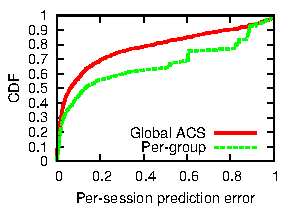
\includegraphics[width=0.3\textwidth] {figures/newfig/example-granular-metric0-new.pdf}
\tightcaption{Comparison of different granular of selection. Per-group ACS selection picks the best ACS in each finest group using history data. Somewhat suprisingly, choosing ACS for each finest group will increase prediction error due to overfitting.}
\label{fig:global-acs}
\end{figure}


To conclude, based on the above empirical analysis, GO's ACS selection searches for best global ACS using greedy algorithm. 

\xil{flow from beginning of sec 5 to this point is VERY CONFUSING}\jc{Is it better now?}

\tightsubsection{Prediction under non-normal data distribution}
\label{subsec:sudo}
The WIMSE algorithm assumes that bias and variance can be computed exactly, while in practice variance cannot be estimated accurately when groups are very small and the sample distribution is not normal. For instance, it is very likely to have all samples in a group with the same values and prediction based on this information will be greatly biased and even worse, WIMSE will treat this group as with zero variance. This is a particularly serious problem for video quality metrics such as buffering ratio and start failure where value of zero is usually dominant.
To alleviate this, we use a simple idea from Bayesian statistics~\cite{}\jc{Henry, give a pointer}: We incorporate a prior distribution on quality outcomes within each group.  This amounts to adding a few fake ``pseudocount'' observations to each group.  Empirically, we see an improvement of at most 5.6\% in prediction error of buffering ratio and 4.5\% in start failure.

\comment{
\begin{figure}[h!]
\centering
 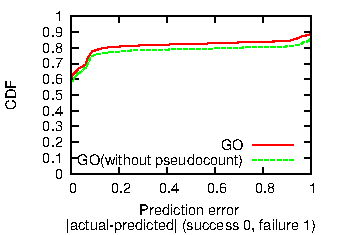
\includegraphics[width=0.4\textwidth] {figures/prediction-comparisons/example-pcount-metric3.pdf}
\tightcaption{GO with pseudocount vs. without pseudocount (considerd quality metric is average bitrate).}
\label{fig:sudocount}
\end{figure}
}

\begin{figure*}[t!]
\centering
\subfigure[Buffering ratio]
{
        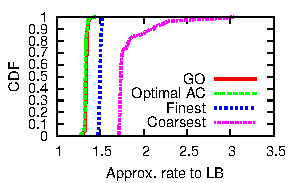
\includegraphics[width=0.25\textwidth]{figures/newfig/example-fig-cdf-all-metricId0.pdf}
}
\hspace{-0.6cm}
\subfigure[Average bitrate]
{
        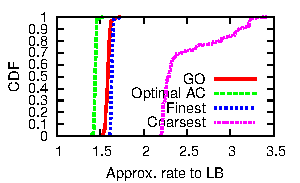
\includegraphics[width=0.25\textwidth]{figures/newfig/example-fig-cdf-all-metricId1.pdf}
}
\hspace{-0.6cm}
\subfigure[Join time]
{
        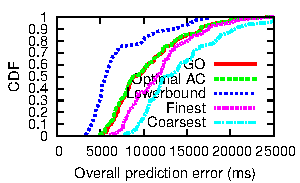
\includegraphics[width=0.25\textwidth]{figures/newfig/example-fig-cdf-all-metricId2.pdf}
}
\hspace{-0.6cm}
\subfigure[Start failure]
{
        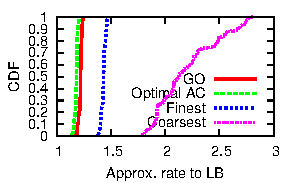
\includegraphics[width=0.25\textwidth]{figures/newfig/example-fig-cdf-all-metricId3.pdf}
}
\tightcaption{Comparison between GO with two oracle approaches (lower bound and optimal AC) and two strawman approaches (finest and coarsest).}
\label{fig:compare-to-naive}
\end{figure*}

\tightsubsection{Comparison with oracle and strawman}
\label{subsec:minieval}

To conclude the section, we compare GO (with ACS selection and pseudocount prior) against two oracle approaches -- the lower bound (\Section~\ref{subsec:lowerbound}) and the optimal AC (\Section~\ref{subsec:aggregation}).  Recall that the optimal AC reflects the best possible prediction using the best AC of historical data based on the quality informaton of sessions under prediction, while the lower bound represents the best possible prediction in theory with no constraint on the way we use historical data. Figure~\ref{fig:compare-to-naive} shows the distribution of overall prediction error at each minute using different methods. It suggests that GO performs very similarly to optimal AC and close to the lower bound (e.g., a difference of \fillme Kbps in average bitrate). 

To put this prediction accuracy into context, we also consider two strawman prediction algorithms that do not use adaptive degree of aggregation.
\begin{packeditemize}
	\item Coarsest AC: Predict using average of each CDN and bitrate combination: picking the decision that is globally best (i.e., no client-side spatial partition)
	\item Finest AC: Predict using average of the finest group that has any data.
\end{packeditemize}

All these results indicate that GO performs better than both strawman, with reduction in prediction accuracy of almost 25+\% from coarsest AC and 1-10\% from finest AC all four metrics. This confirms the observation in \Section~\ref{subsec:aggregation} that the best level of aggregation is often dynamic and in between the coarsest and finest aggregation.


Finally, we revisit the observation on the variability of the lower bound across different ASN and Site. Figure~\ref{fig:compare-partition} picks the largest 3 Sites and compare GO's prediction accuracy with baseline (Coarsest) as well as the lower bound. As shown, with the lower bound varying across different Site, GO can always achieve close-to-optimal prediction accuracy (i.e., low overall prediction error).

\begin{figure}[h!]
\centering
\subfigure[Buffering ratio]
{
        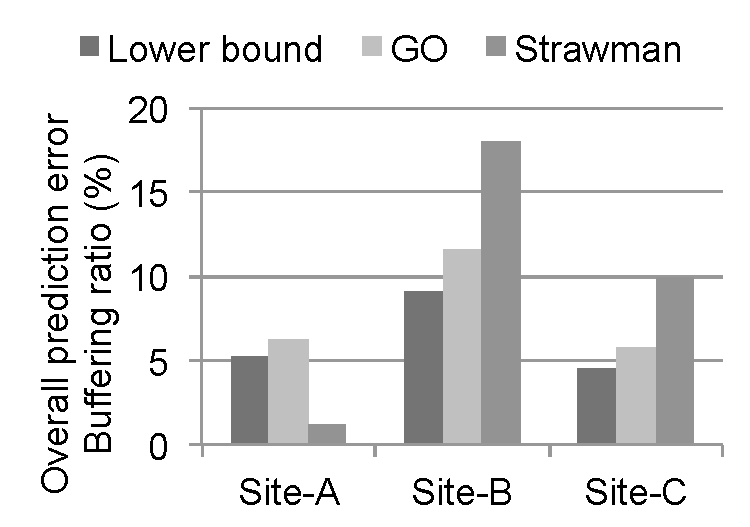
\includegraphics[width=0.24\textwidth]{figures/newfig/bar-compare-bufratio.pdf}
}
\hspace{-0.6cm}
\subfigure[Average bitrate]
{
        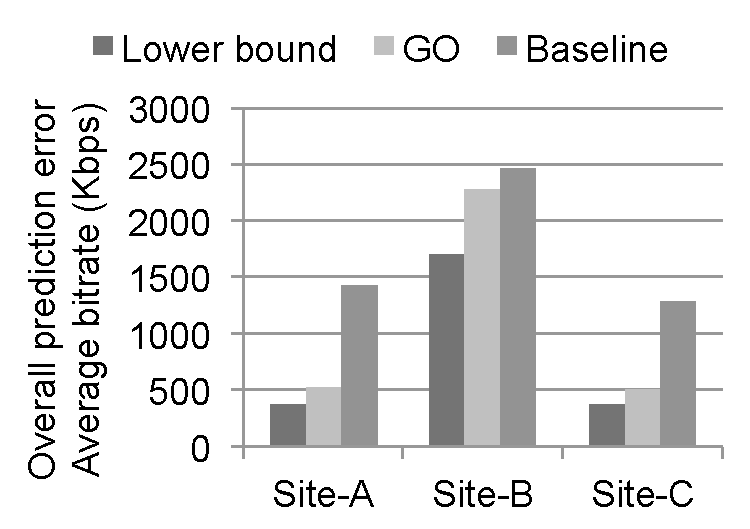
\includegraphics[width=0.24\textwidth]{figures/newfig/bar-compare-bitrate.pdf}
}
\tightcaption{Comparison of prediction error between GO, lower bound and baseline (coarsest AC) in different partitions.}
\label{fig:compare-partition}
\end{figure}

\comment{
\tightsubsection{Interactions between decisions\jc{Move to discussion}}
The reader may be bothered by a simplifying assumption implicit in our characterization of the causes of prediction error.  If we allocated all traffic to a single CDN, its performance might degrade, but our session-wise prediction does not capture that.  We might instead want to know the following: Given a set of decisions about sessions (say, all the sessions we observe in a 1-hour interval), what is the predicted performance for that set of sessions?  We do not wish to say that such a question is impossible to answer, but rather point out some difficulties in answering it, and some reasons why it is less critical to answer it than it may appear.

Joint prediction is statistically difficult because existing statistical prediction algorithms typically assume the performance of training examples are independent and experience identical randomness (i.e. they are IID).  We observe very few IID instances of whole sets of sessions; in our example, we observe only one per 1-hour interval.  It is possible to model explicitly the dependence of each session’s performance on the set of joint decisions, but this requires modeling choices that we may not make well, and such models are typically computationally expensive to learn. \fillme

If conditions change slowly enough, the independence assumption is not so bad.
The rate of change of CDN allocations is naturally limited for our problem by the rate of session arrivals, since we choose CDNs only at the beginning of each session.  Spikes in the rate of new sessions are not typically high enough to necessitate special handling.  \henry{Need some data and experiments for this.  Davis or Florin have done some of the experiments, I think.}


\tightsubsection{Alternative approaches\jc{Move to discussion}}
The reader should not leave with the impression that the algorithm described above is the only possible one for predicting video quality, or even the best.  The scope of this paper is merely to establish a reasonable approach and show that it results in improvements.  Other possible approaches might include:
\begin{packedenumerate}
  \item \emph{Linear regression:} After encoding categorical attributes as binary features, simple linear regression can be applied to predict quality outcomes.  Temporal attributes can be passed through nonlinear functions to achieve reasonable time-series prediction.  Interaction terms (e.g. the indicator for a session coming from ASN $100$ multiplied by the indicator for the session having Object ``foo'') can simulate attribute combinations, at the cost of a combinatorial explosion in the size of the learned model.  However, recent developments in optimization for $\ell_1$-regularized linear regression allow models to be learned quickly online while providing the guarantee that the learned model is \emph{sparse}, i.e. that only a few important features are selected for inclusion in the model and the rest can be safely dropped.  See \cite{duchi2010composite} for one example of work that could enable this technique.  One downside is that linear models are harder to interpret than a model based on averaging group averages.
  \item \emph{Hierarchical Bayesian modeling:} In this approach, groups are placed in the natural tree, and each is associated with a probability distribution over quality outcomes, such as a Gaussian distribution.  Each group inherits information from the distribution of its parent group in the form of a prior.  Such models potentially deal very naturally with data sparsity and with dependence among sessions \cite{gelman2003bayesian}, but learning them from data is often computationally intractable.
\end{packedenumerate}
}
